% !TeX root = ../main.tex
% Add the above to each chapter to make compiling the PDF easier in some editors.

\chapter{Introduction}\label{chapter:introduction}

For the entirety of recent history, \acrlong{AR} has been a staple of science fiction stories, regardless of their setting or of the medium used to portray them, be it written text, pictures, movies or video-games. This concept is so ingrained in popular culture that almost every technology enthusiast or sci-fi aficionado has a mental image of how a system using it could look like.

What is less known is that \acrlong{AR} prototypes have been a reality for a long time, since the late 1970s\cite{kocian_visually-coupled_1977}. However, those early systems were difficult to use, as they required expensive devices and lengthy calibration procedures. This effectively restricted them to military research environments and, later, university research laboratories.

Luckily, this is not the case anymore: in the last ten years the \gls{AR} field has moved forward very quickly, thanks to the fact that current-generation mobile devices pack enough performance to support these use cases and thanks to the commercialization of the associated field of \gls{VR}, which finally has become available as an off-the-shelf product. This in turn caught the interest of big players like Microsoft, Apple, Google, Meta and others, which have been doing a lot of the work that is necessary to transform \gls{AR} from a research \enquote{novelty} to a platform easily accessible by developers with a less specific background\cite{google_llc_arcore_nodate, apple_inc_arkit_nodate, microsoft_corporation_microsoft_nodate, meta_platforms_inc_spark_nodate}.

The first concrete proofs of these advancements have been \gls{AR} video-games like PokemonGO\cite{niantic_inc_pokemon_nodate}, which for the first time have brought an (admittedly limited) \acrlong{AR} experience to the general public, and the integration of an high-level \gls{AR} \gls{API} in most of the major platforms, from the Unity game engine\cite{unity_technologies_unity_nodate} to WebXR\cite{world_wide_web_consortium_webxr_nodate}. The most interesting result of the renaissance of this field has been the development of \gls{AR} \glspl{HMD} like the Microsoft Hololens\cite{microsoft_corporation_microsoft_nodate} (shown in \autoref{fig:hololens_image}) and the Magic Leap One \cite{magic_leap_inc_magic_nodate}. For the first time, they allow the development of \gls{AR} experiences that are very close to the ideal ones imagined in science fiction stories, as such devices are fairly comfortable to wear, do not require lengthy calibrations, are capable of overlaying augmentations on a decent portion of the wearer's \gls{FOV} and are self-contained, meaning that they do not require external tethers.

\begin{figure}
  \centering
  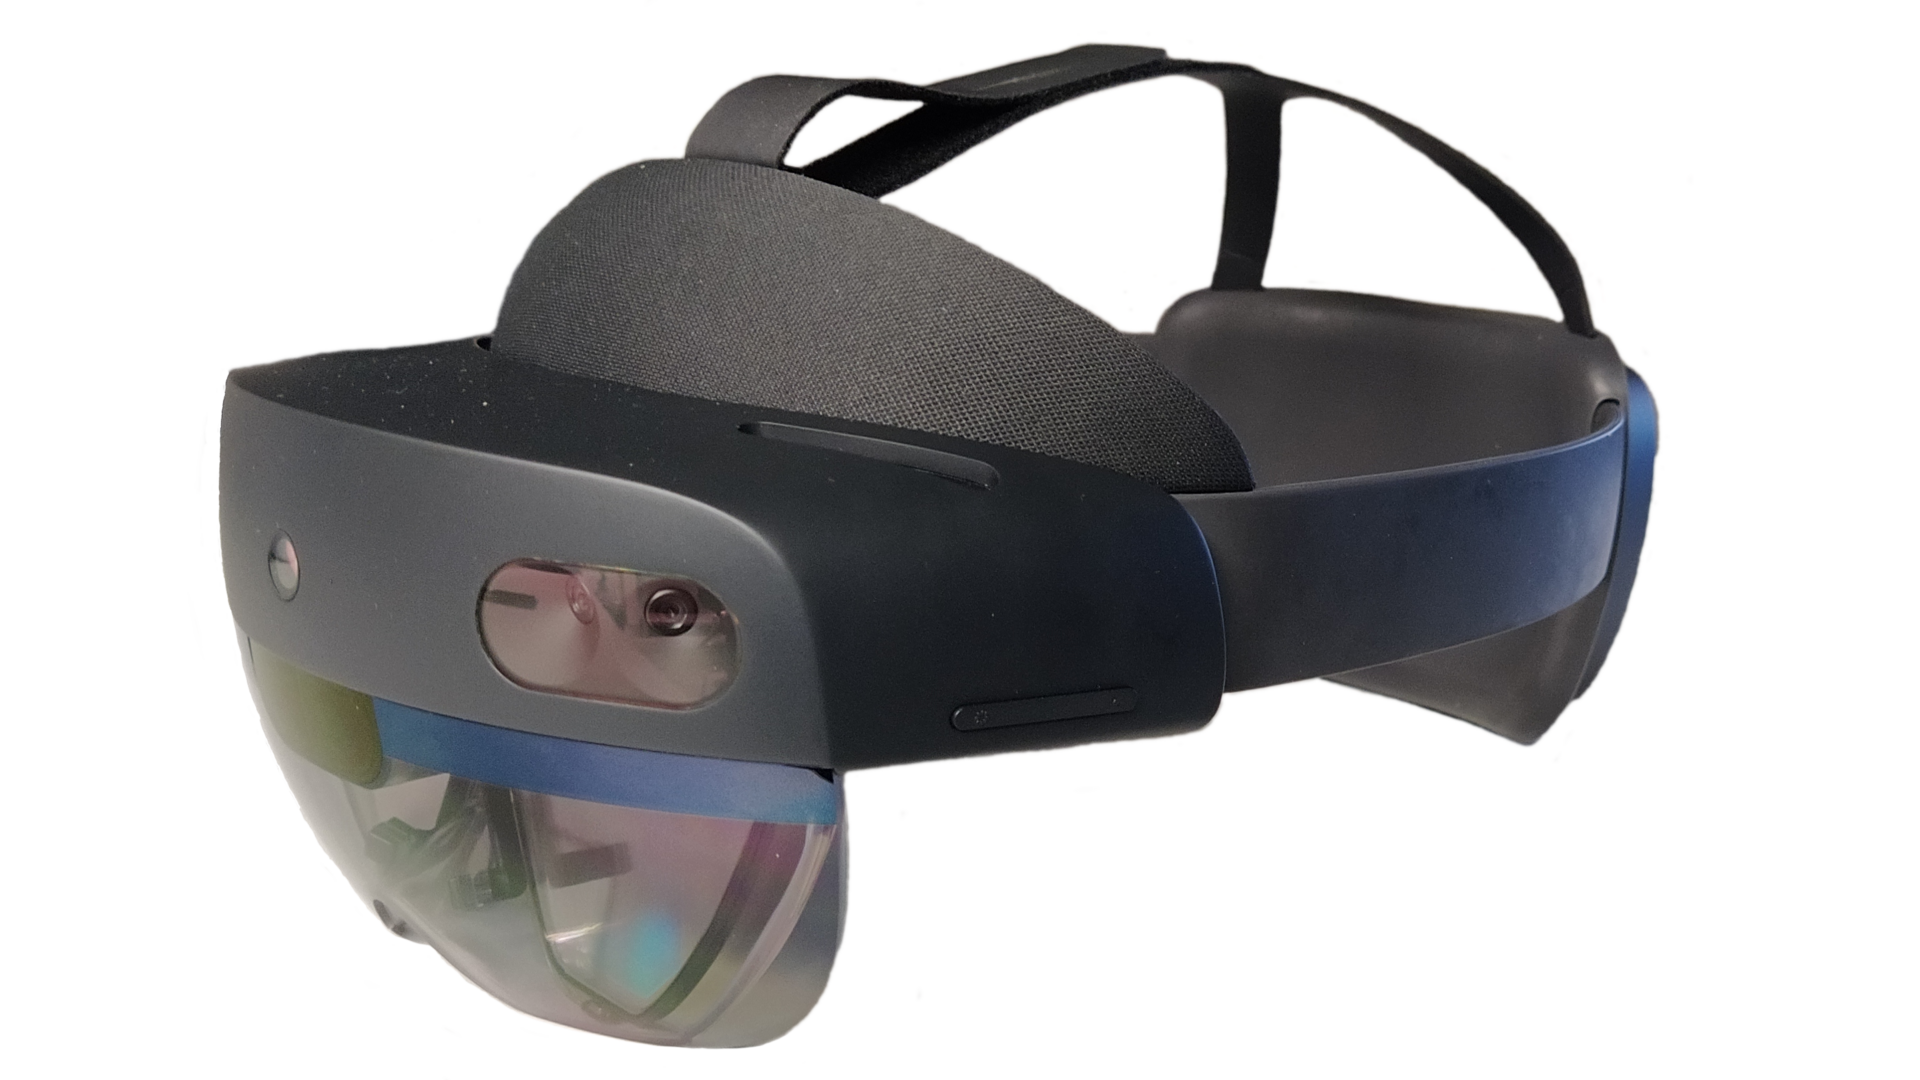
\includegraphics[width=0.6\textwidth]{hololens.png}
  \caption{The Microsoft Hololens 2.}\label{fig:hololens_image}
\end{figure}

This hardware availability alone already offers many possibilities for developers and researchers wanting to experiment with \gls{AR}, as these devices are cheaper and easier to use than what was previously available as a commercial product. However, another significant part of these improvements regards how developers interface with such devices: although \glspl{HMD} have existed for a while, they often offered a very low level \gls{API} that only allowed to specify the color of each individual pixel of the display. In order to obtain an AR-capable system, the developer had to acquire the information coming from an external tracker, process it and then generate the correct 2D image to be displayed on such \gls{HMD}, which is non-trivial and requires a significant amount of software engineering work. A concrete example of this is the current version of the ROSIE\cite{viertler_requirements_2015} rotorcraft simulator, which uses a custom C++ 3D engine that integrates the pose information coming from an external tracker and the description of the desired virtual 3D scene to produce an image that is then used to drive the individual pixels of an old-generation \gls{HMD}. Besides the initial development cost, this kind of setup also presents recurring costs, as new developers and researchers need to become familiar with a fairly complex setup, and often end up spending a significant amount of time on software engineering issues rather than their original research question.

Devices like the Hololens eliminate a meaningful portion of this complexity, as they abstract away the inner workings of the tracking system and other implementation details to offer a higher-level platform that explicitly targets the development of \gls{AR} applications. Moreover, the industry decided to converge early on a device-independent \gls{API} called OpenXR\cite{world_wide_web_consortium_webxr_nodate}, which allows developers to write their application once and then be able to run it on a multitude of different \gls{AR} devices. This caught the interest of game engine designers, who saw an easy opportunity to extend their platform to also support OpenXR as a target, leading to the current situation in which one can quickly write a Hololens application in Unity, enjoying the features of a modern game engine, without having to focus too much on the low-level details of how the Hololens actually works. This allows developers and researchers to shift their focus from \emph{building} an \gls{AR} system to just \emph{using} an \gls{AR} system, allowing them to pursue their research question rather than work on software engineering issues.

\section{Related work}\label{section:relatedwork}

Concrete evidences of these recent developments are readily available. Not only devices like the Microsoft Hololens\cite{microsoft_corporation_microsoft_nodate} and the Magic Leap One\cite{magic_leap_inc_magic_nodate} are commercially available, they are already being put to use. An example is the field of medical augmented reality, where researches are using the Hololens to aid the positioning of complex medical machinery\cite{andress_--fly_2018, fotouhi_interventional_2016, fallavollita_desired-view--controlled_2014} and train surgeons in complex procedures\cite{turini_microsoft_2018}. The Hololens has also already been used with success in real human surgeries\cite{assistance_publique_hopitaux_de_paris_world_nodate}. Another example is the suite of commercially available \gls{AR} applications available for use on the Hololens 2, both offered by Microsoft themselves\cite{microsoft_corporation_remote_nodate} and by third parties\cite{microsoft_corporation_apps_nodate}. A last example is given by the \gls{AR} experiences already developed for rotorcraft simulators, which show promising results in highlighting obstacles and displaying approach paths\cite{walko_increasing_2021}. Exploration is happening also in the direction of single-pilot cockpits\cite{tran_single_2018}.

\section{Problem statement}\label{section:problemstatement}
Aircrafts are complex environments with a low tolerance for errors. Pilots have to monitor a number of different flight parameters while at the same time having to fly the aircraft, navigate the planned route and communicate with an external traffic control entity. Especially in abnormal situations, this requires deep knowledge of the aircraft and quick decision-making skills. Moreover, there is the risk of \enquote{cognitive overload}, in which the pilot has to deal concurrently with too many information, which could lead to missing an important data point with potentially severe consequences.

A reasonable hypothesis is that a part of the complexity of these situations is accidental\cite{brooks_no_1987} and that it is due to how the information is presented to the pilot. The design of aircraft cockpits and their interfaces with the pilot have been studied for many years and are therefore already highly optimized for safety and clarity, making further improvements difficult to achieve. However, research focused primarily on improving standard and well-known technologies, like normal displays, gauges, switches and buttons. Due to the limitations mentioned at the beginning of \autoref{chapter:introduction}, experimenting with \gls{AR} solutions in these contexts has been difficult, with available \glspl{HMD} solutions being cumbersome to setup and/or being limited to displaying only 2D elements like speed and altitude, as shown in \autoref{fig:traditional_hmd_view.png}.

\begin{figure}
  \centering
  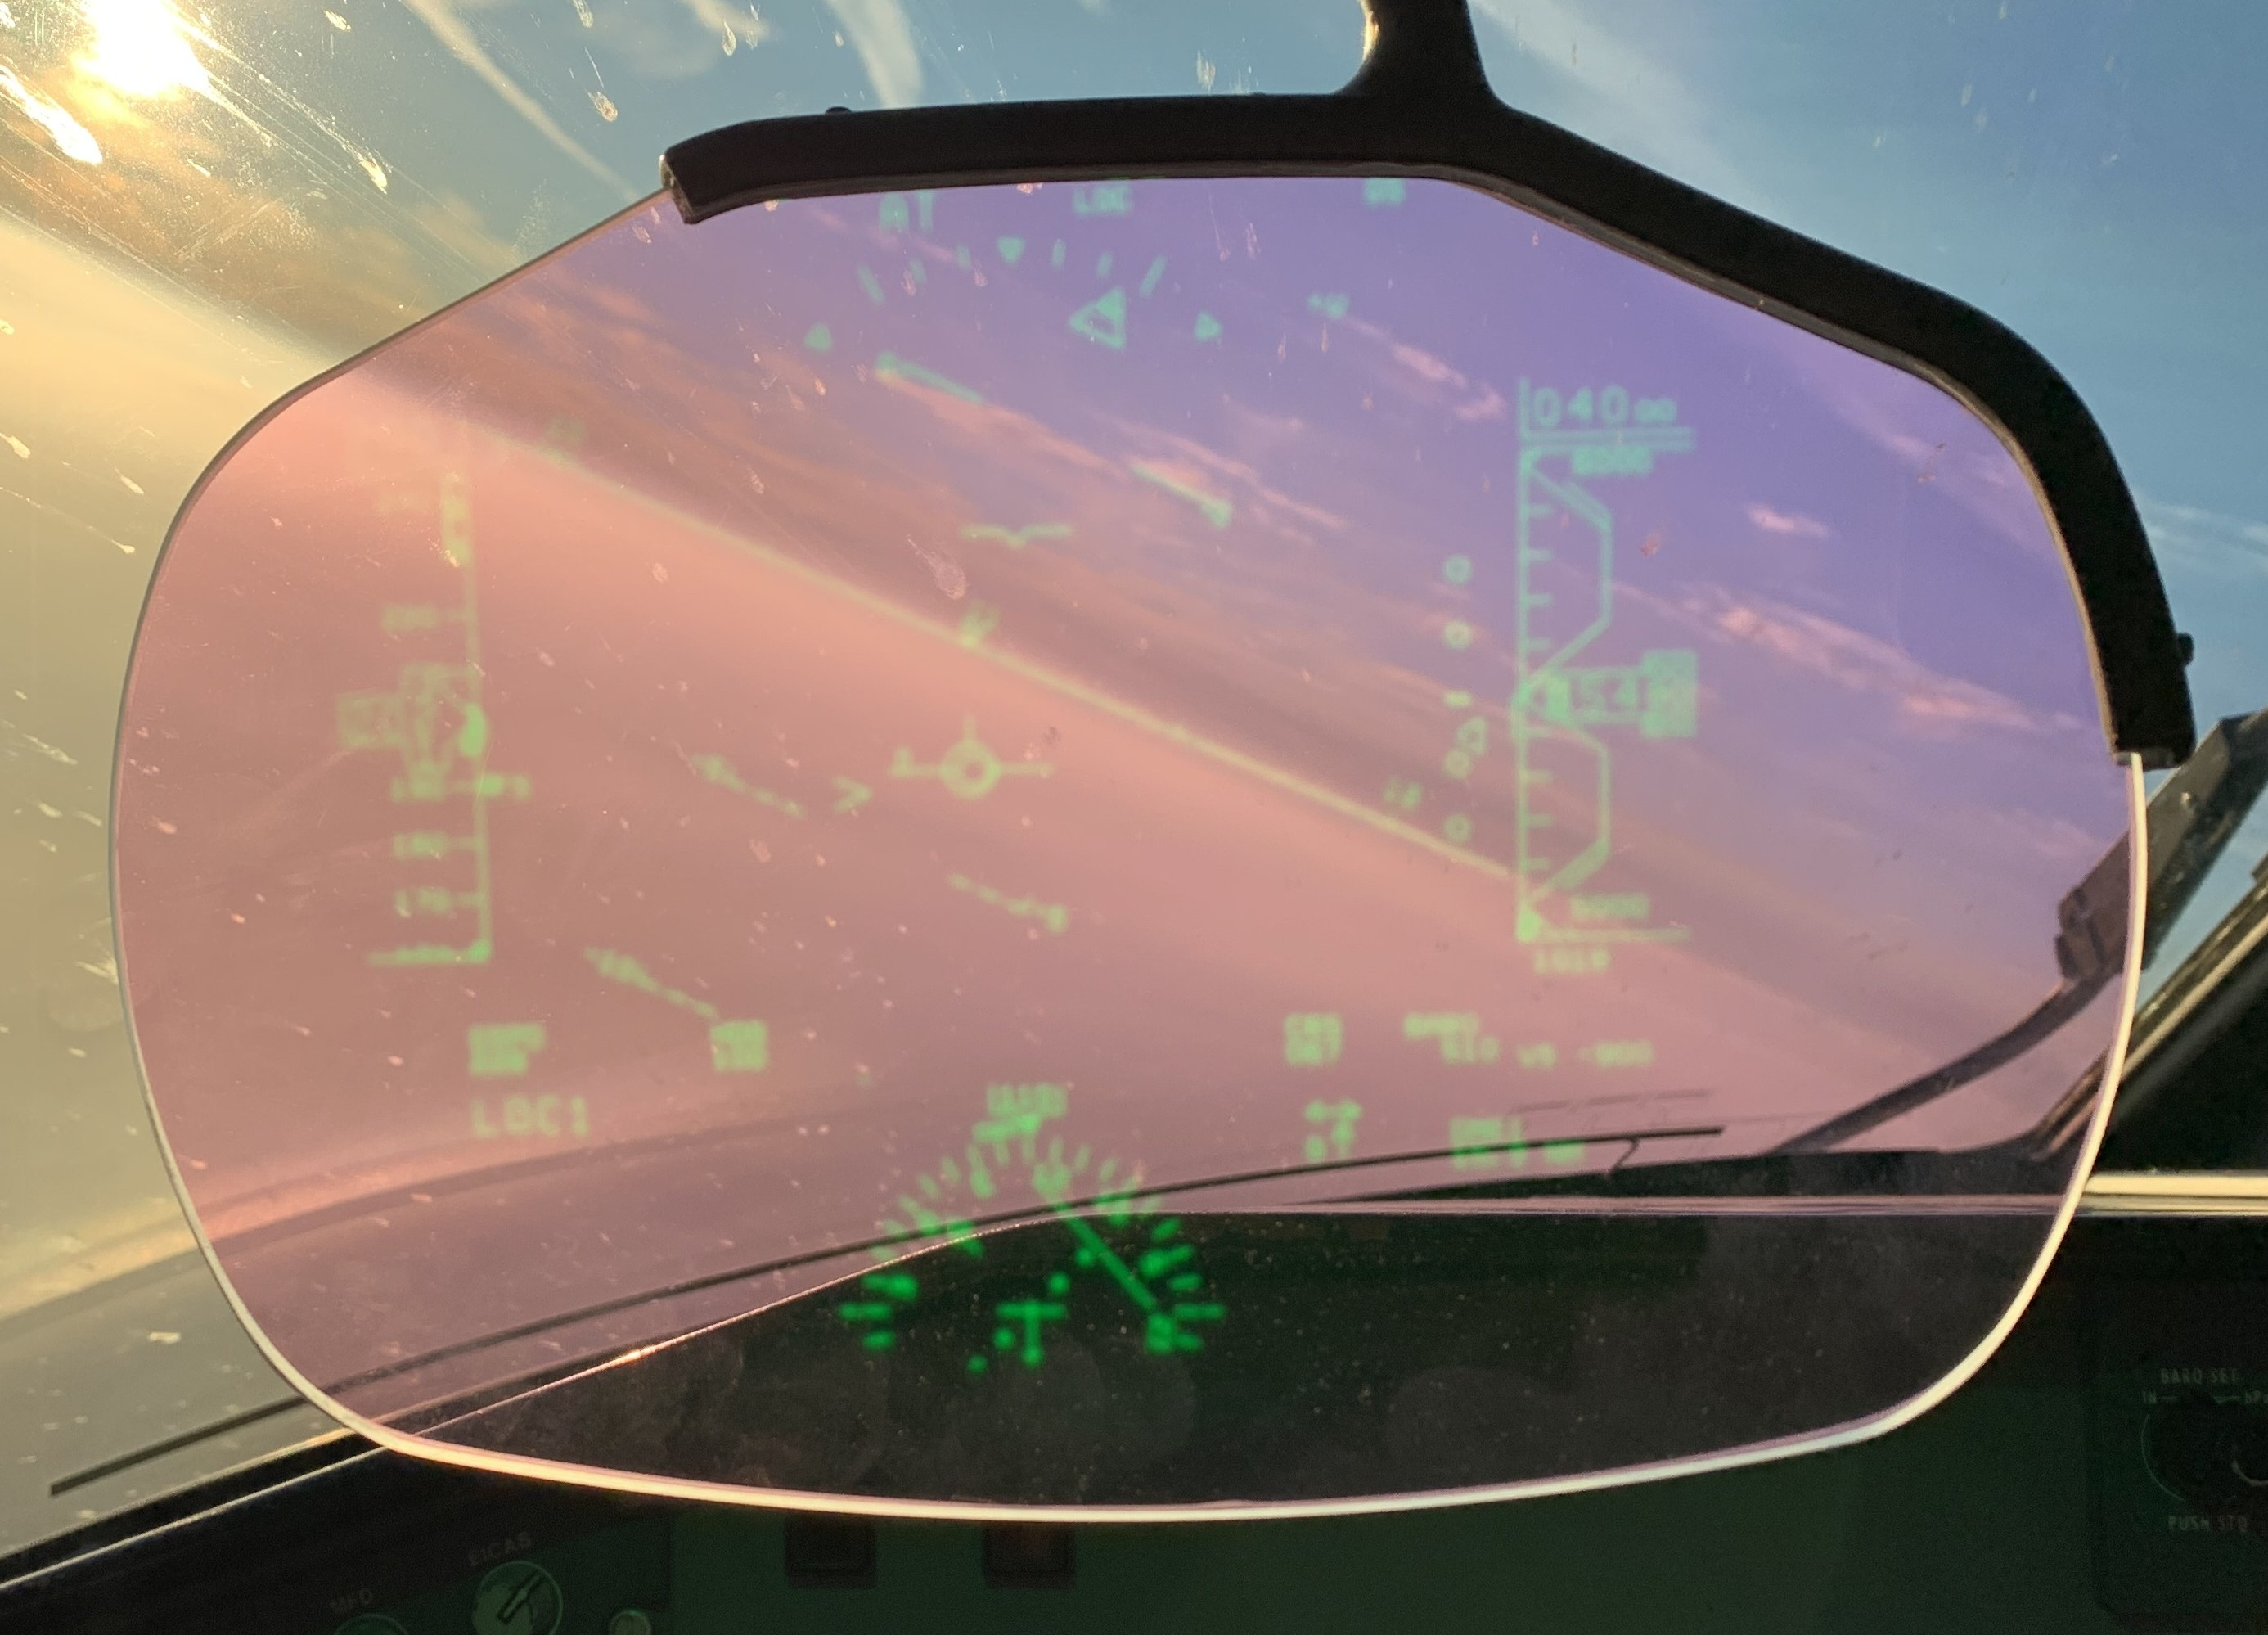
\includegraphics[width=0.6\textwidth]{traditional-hmd-view.jpg}
  \caption{The view shown by a traditional \gls{HUD}, composed only of 2D elements.}\label{fig:traditional_hmd_view.png}
\end{figure}

The recent availability of devices like the Microsoft Hololens has sparked interest in this area, especially as far as rotary-wing aircrafts are concerned\cite{walko_integration_2020, walko_increasing_2021}. Since \acrlong{AR} experiences aim to blend seamlessly with the way humans usually experience reality, there are well-justified hopes that they will represent the next step in user interface and user experience design, as they should be significantly more intuitive to use than traditional display-based solutions. If this turns out to be true, then \gls{AR} could be used to present information to pilots in a more efficient way, leading to even safer flight conditions.

Another context in which \gls{AR} could potentially be beneficial are \glspl{eVTOL}: they will probably be commanded by a single pilot with limited training, who will therefore require all the assistance that technology can possibly offer.

The only way to prove (or disprove) this belief in \acrlong{AR} is to use modern \gls{AR} \glspl{HMD} first in simulators and then in real aircrafts. New, more advanced visualizations will have to be shown to pilots and their feedback on whether these solutions are better or worse than what is currently available will have to be collected. In order to do this, it must be as easy as possible to create \gls{AR} experiences for flight simulators, to enable a rapid feedback cycle that will allow to test many different visualization ideas and to iterate on them quickly. Moreover, developing these \gls{AR} experiments should require as little programming knowledge as possible, because researchers working on them will likely have very different backgrounds and a varying level of computer science expertise. 

To achieve this objective, the appropriate tooling and workflows to create these \gls{AR} experiences have to be developed, and this is the main aim of this thesis. Moreover, to show that the resulting platform is actually helpful, an initial \gls{AR} experience will be developed and presented to a small sample of experienced pilots, who will give an assessment of its usefulness. The aim of such experiment will be to create \gls{AR} augmentations that help pilots to land at the Innsbruck airport in condition of limited visibility, as that landing is comparatively more difficult than many others due to the orographic formations that surround the airport. The developed tooling consist mainly of two parts:

\begin{enumerate}
    \item \enquote{\gls{holoassist}}, a Unity application that runs on the Hololens and contains most of the logic required to display 3D augmentations in the setting of a flight simulator. 
    \item \enquote{\glspl{holoassistapp}}, a collection of scripts that use the \gls{API} exposed by \gls{holoassist} to draw the augmentations that have to be shown to the pilot in the context of an experiment.
\end{enumerate}

\textbf{TL;DR.} In order to evaluate whether \gls{AR} solutions are actually helpful in the context of an aircraft cockpit there is the need to quickly build \gls{AR} experiences and test them on a flight simulator. This thesis project builds the tooling and workflow needed to achieve these capabilities.

\section{Technical limitations}
Although devices like the Hololens seem very promising, they are still targeted mostly for research environments and experimentation, as they still have rough edges and limitations, especially for more exotic use cases like the one presented in this document. First of all, they have a limited battery life (about two hours of actual usage on the Hololens 2): using current iterations of these devices in a real aircraft will therefore require some integration with the airplane's electrical system in order to keep them charged. Additionally, the computing power available on-device is fairly constrained, which limits the complexity of the augmentations that can be shown.

The Hololens also has a pretty significant problem specific to the use case presented in these pages. The inside-out tracking relies heavily on an \gls{IMU} embedded in the device. This means that whenever the device is used on a moving platform (like a car, a ship or an aircraft) the tracking is sub-optimal and often lost completely, making the device unusable. The eventual desire is to be able to show augmentations while being in full-motion flight simulators and in real aircrafts, but this will not be possible with the current iteration of the Hololens (unless an external tracking system is used, with all the complexity that it would entail). Fortunately, Microsoft is aware of this issue and working on a solution\cite{microsoft_corporation_hololens_nodate}, which however is currently only effective only for low-jerk motions like those of a cruise ship (rather than the sudden changes in acceleration of a sport car).

\section{Thesis overview}

The remainder of this document describes the proposed solution for the problem statement expressed in \autoref{section:problemstatement}. Chapter \ref{chapter:holoassist} deals with the Hololens side of the solution: each section focuses on a different problem that \gls{holoassist} had to solve in order to display the desired augmentations. A particular mention goes to \autoref{section:geofixedaugmentations}, which explains how such augmentations are represented in memory and rendered, which is arguably the most complex part of the Hololens application. Chapter \ref{chapter:holoassistapps} describes how \gls{holoassist}'s \gls{API} can be used to create \gls{AR} experiences inside a fixed-platform simulator and what was implemented to enhance the landing at Innsbruck's airport. Chapter \ref{chapter:evaluation} describes how the quality of the augmentations developed for Innsbruck's airport was assessed and \autoref{chapter:conclusions_and_future_work} summarizes the main outcomes of the whole project and some potential future steps.

Additional content is available in the appendices, which contain a detailed documentation of the \gls{holoassist} \gls{API} and a semi-serious description of some of the more puzzling bugs that were encountered during the development of the Hololens application.